\documentclass[a4paper]{article}
\usepackage[margin=1.5cm]{geometry}
\usepackage{amsmath}
\usepackage{amssymb}
\usepackage{enumitem}
\usepackage{tikz}
\usepackage{url}
\usetikzlibrary{matrix}
\begin{document}
\pagestyle{empty}

\begin{center}
    {\LARGE \textbf{Tugas Personel ke-2}}\\[0.5em]
    {\Large \textbf{Week 7}}
\end{center}

\begin{enumerate}[itemsep=1em,leftmargin=*]
  \item Cari semua turunan parsial kedua dari persamaan Berikut (LO1, max point = 20)
  \begin{enumerate}[itemsep=1em]
    \item \(f(x,y) = x^4y - 2x^3y^2\)

    Mencari turunan parsial pertama terhadap \(x\) dan \(y\) dari fungsi \(f(x,y)\) terlebih dahulu:

    \begin{enumerate}[itemsep=1em,leftmargin=*]
        \item \(f_x = \frac{\partial f}{\partial x}\)

        \(f(x,y) = x^4y - 2x^3y^2\)

        \(f_x = 4x^3y - 6x^2y^2\)

        \item \(f_y = \frac{\partial f}{\partial y}\)

        \(f(x,y) = x^4y - 2x^3y^2\)

        \(f_y = x^4 - 4x^3y\)

    \end{enumerate}

    Untuk semua turunan parsial kedua, diambil dari \(f_x\) dan \(f_y\):

    \begin{enumerate}[itemsep=1em,leftmargin=*]
        \item \(f_{xx} = \frac{\partial^2 f}{\partial x^2} = \frac{\partial f_x}{\partial x}\)

        \(f_x = 4x^3y - 6x^2y^2\)

        \(f_{xx} = 12x^2y - 12xy^2\)

        \item \(f_{yy} = \frac{\partial^2 f}{\partial y^2} = \frac{\partial f_y}{\partial y}\)

        \(f_y = x^4 - 4x^3y\)

        \(f_{yy} = -4x^3\)

        \item \(f_{xy} = \frac{\partial^2 f}{\partial x \partial y} = \frac{\partial f_x}{\partial y}\)

        \(f_x = 4x^3y - 6x^2y^2\)

        \(f_{xy} = 4x^3 - 12x^2y\)

        \item \(f_{yx} = \frac{\partial^2 f}{\partial y \partial x} = \frac{\partial f_y}{\partial x}\)

        \(f_y = x^4 - 4x^3y\)

        \(f_{yx} = 4x^3 - 12x^2y\)
    \end{enumerate}

    \item \(z = \frac{y}{2x+3y}\)

    Mencari turunan parsial pertama terhadap \(x\) dan \(y\) dari fungsi \(z\) terlebih dahulu menggunakan \textbf{aturan hasil bagi} (\textbf{Quotient rule}):

    \(f'(x) = \frac{u'(x)v(x) - u(x)v'(x)}{[v(x)]^2}\)

    \begin{enumerate}[itemsep=1em,leftmargin=*]
        \item \(z_x = \frac{\partial z}{\partial x}\)

        \(z = \frac{y}{2x+3y}\)

        \(z_x = \frac{(0)(2x+3y) - (y)(2)}{(2x+3y)^2} = \frac{-2y}{(2x+3y)^2}\)

        \item \(z_y = \frac{\partial z}{\partial y}\)

        \(z = \frac{y}{2x+3y}\)

        \(z_y = \frac{(1)(2x+3y) - (y)(3)}{(2x+3y)^2} = \frac{2x + 3y - 3y}{(2x+3y)^2} = \frac{2x}{(2x+3y)^2}\)
    \end{enumerate}

    Untuk semua turunan parsial kedua, diambil dari \(z_x\) dan \(z_y\) menggunakan \textbf{aturan hasil bagi}, \textbf{aturan rantai} (\textbf{Chain rule}), dan \textbf{aturan perkalian} (\textbf{Product rule}):

    \vspace{1em}

    \textbf{Aturan rantai} (\textbf{Chain rule})
    
    \(\frac{dy}{dx} = f'(g(x)) \cdot g'(x)\)

    \(\frac{\partial z}{\partial x} = \frac{\partial z}{\partial u} \cdot \frac{\partial u}{\partial x}\)

    \textbf{Aturan perkalian} (\textbf{Product rule})
    
    \(\frac{dy}{dx} = u'(x)\,v(x) + u(x)\,v'(x)\)

    \(\frac{\partial (uv)}{\partial x} = u_x v + u v_x\)

    \vspace{1em}

    \begin{enumerate}[itemsep=1em,leftmargin=*]
        \item \(z_{xx} = \frac{\partial^2 z}{\partial x^2} = \frac{\partial z_x}{\partial x}\)

        \(z_x = \frac{-2y}{(2x+3y)^2}\)

        \(z_{xx} = \frac{(0)(2x+3y)^2 - (-2y)(4)(2x+3y)}{(2x+3y)^4} = \frac{8y(2x+3y)}{(2x+3y)^4} = \frac{8y}{(2x+3y)^3}\)

        \item \(z_{yy} = \frac{\partial^2 z}{\partial y^2} = \frac{\partial z_y}{\partial y}\)

        \(z_y = \frac{2x}{(2x+3y)^2}\)

        \(z_{yy} = \frac{(0)(2x+3y)^2 - (2x)(6)(2x+3y)}{(2x+3y)^4} = \frac{-12x(2x+3y)}{(2x+3y)^4} = \frac{-12x}{(2x+3y)^3}\)

        \item \(z_{xy} = \frac{\partial^2 z}{\partial x \partial y} = \frac{\partial z_x}{\partial y}\)

        \(z_x = \frac{-2y}{(2x+3y)^2}\)

        \(z_{xy} = \frac{(-2)(2x+3y)^2 - (-2y)(6)(2x+3y)}{(2x+3y)^4}\)

        \(z_{xy} = \frac{(2x+3y)[-2(2x+3y) + 12y]}{(2x+3y)^4}\)

        \(z_{xy} = \frac{(2x+3y)(-4x + 6y)}{(2x+3y)^4}\)

        \(z_{xy} = \frac{-4x+6y}{(2x+3y)^3}\)

        \item \(z_{yx} = \frac{\partial^2 z}{\partial y \partial x} = \frac{\partial z_y}{\partial x}\)

        \(z_y = \frac{2x}{(2x+3y)^2}\)

        \(z_{yx} = \frac{(2)(2x+3y)^2 - (2x)(4)(2x+3y)}{(2x+3y)^4}\)

        \(z_{yx} = \frac{(2x+3y)[2(2x+3y) - 8x]}{(2x+3y)^4}\)

        \(z_{yx} = \frac{(2x+3y)(-4x + 6y)}{(2x+3y)^4}\)

        \(z_{yx} = \frac{-4x+6y}{(2x+3y)^3}\)

    \end{enumerate}
  \end{enumerate}
  \item Jelaskan F dan buat sketsa beberapa vektor dalam medan vektor F(x,y) yang diberikan oleh (LO1, max point = 20)
  \begin{enumerate}[itemsep=1em]
    \item \(f(x,y) = xi + \frac{1}{2}yj\)
    
    Dari fungsi \(f(x,y) = xi + \frac{1}{2}yj\), kita dapat mengekstrak komponen-komponen vektor sebagai berikut:

    \[
    \begin{array}{l|l|l}
    (x, y) & \mathbf{F}(x,y) = \langle x, \tfrac{1}{2}y \rangle & \text{Keterangan arah} \\ \hline
    (-3,\, 1.5) & \langle -3,\, 0.75 \rangle & \text{Ke kiri atas} \\
    (-1.5,\,-2) & \langle -1.5,\,-1 \rangle & \text{Ke kiri bawah} \\
    (0.5,\, 3) & \langle 0.5,\, 1.5 \rangle & \text{Ke kanan atas} \\
    (1.5,\,-0.5) & \langle 1.5,\,-0.25 \rangle & \text{Ke kanan bawah} \\
    (3,\, 0.5) & \langle 3,\, 0.25 \rangle & \text{Ke kanan (hampir datar)} \\
    \end{array}
    \]

    \vspace{1em}

    \begin{center}
    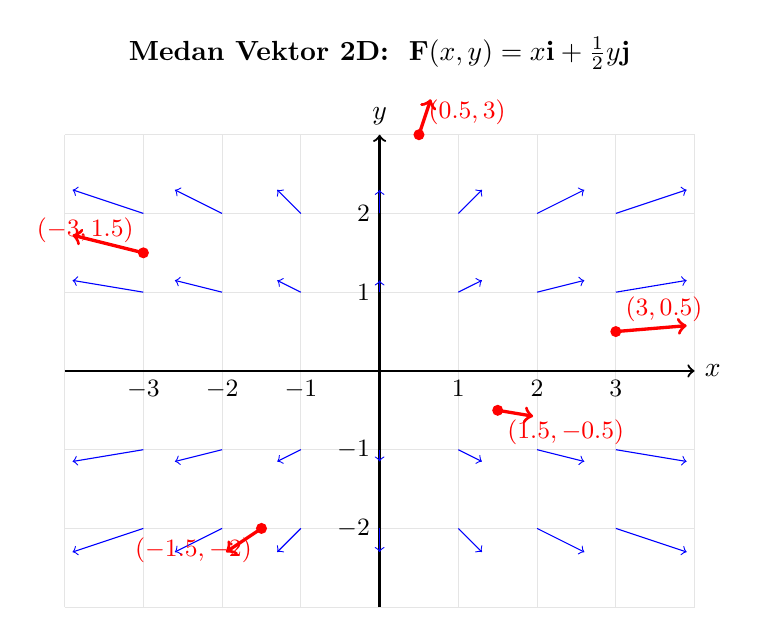
\begin{tikzpicture}[scale=1.0]
        \draw[gray!20, step=1] (-4,-3) grid (4,3);
        
        \draw[thick,->] (-4,0) -- (4,0) node[right] {$x$};
        \draw[thick,->] (0,-3) -- (0,3) node[above] {$y$};
        
        \foreach \x in {-3,-2,-1,1,2,3}
            \node[below] at (\x,0) {\small $\x$};
        \foreach \y in {-2,-1,1,2}
            \node[left] at (0,\y) {\small $\y$};
        
        \foreach \x in {-3,-2,-1,1,2,3}
        \foreach \y in {-2,-1,1,2}
        {
            \pgfmathsetmacro{\vx}{\x}
            \pgfmathsetmacro{\vy}{\y/2}
            \draw[->,blue] (\x,\y) -- (\x+0.3*\vx,\y+0.3*\vy);
        }
        
        \draw[->,blue] (0,-2) -- (0,-2.3);
        \draw[->,blue] (0,-1) -- (0,-1.15);
        \draw[->,blue] (0,1) -- (0,1.15);
        \draw[->,blue] (0,2) -- (0,2.3);
        
        \draw[->,red,very thick] (-3,1.5) -- (-3.9,1.725);
        \draw[->,red,very thick] (-1.5,-2) -- (-1.95,-2.3);
        \draw[->,red,very thick] (0.5,3) -- (0.65,3.45);
        \draw[->,red,very thick] (1.5,-0.5) -- (1.95,-0.575);
        \draw[->,red,very thick] (3,0.5) -- (3.9,0.575);
        
        \fill[red] (-3,1.5) circle (2pt) node[above left] {\small $(-3,1.5)$};
        \fill[red] (-1.5,-2) circle (2pt) node[below left] {\small $(-1.5,-2)$};
        \fill[red] (0.5,3) circle (2pt) node[above right] {\small $(0.5,3)$};
        \fill[red] (1.5,-0.5) circle (2pt) node[below right] {\small $(1.5,-0.5)$};
        \fill[red] (3,0.5) circle (2pt) node[above right] {\small $(3,0.5)$};
        
        \node[above] at (0,3.7) {\textbf{Medan Vektor 2D: } $\mathbf{F}(x,y) = x\mathbf{i} + \frac{1}{2}y\mathbf{j}$};
    \end{tikzpicture}
    \end{center}

    Vektor dua dimensi ditulis sebagai:

    \(\mathbf{F}(x, y) = P(x, y)\mathbf{i} + Q(x, y)\mathbf{j}\)

    Dengan soal:

    \(\mathbf{F}(x, y) = x\mathbf{i} + \tfrac{1}{2}y\mathbf{j}\)

    Maka:

    \(P(x, y) = x, \quad Q(x, y) = \tfrac{1}{2}y\)

    \begin{itemize}
      \item $P(x, y)$ adalah komponen arah \textbf{sumbu-$x$ (horizontal)},
      \item $Q(x, y)$ adalah komponen arah \textbf{sumbu-$y$ (vertikal)}.
    \end{itemize}

    Dari sketsa vektor, dapat dikatakan:

    \begin{enumerate}[itemsep=1em,leftmargin=*]
      \item \(x\), arah horizontal dari vektor.
      \item \(\frac{1}{2}y\), arah vertikal dari vektor, tetapi dengan laju yang lebih lambat (setengah dari \(y\)).
      \item Vektor-vektor akan menjauh dari pusat, sehingga dapat dikatakan vektor ini bersifat \textbf{linear} dan \textbf{divergen}.
    \end{enumerate}

    \vspace{1em}

    \item \(f(x,y) = yi + (x+y)j\)

    Dari fungsi \(f(x,y) = yi + (x+y)j\), kita dapat mengekstrak komponen-komponen vektor sebagai berikut:

    \[
    \begin{array}{l|l|l}
    (x, y) & \mathbf{F}(x, y) = \langle y,\, x + y \rangle & \text{Keterangan arah} \\ \hline
    (-3,\, 1.5) & \langle 1.5,\, -1.5 \rangle & \text{Ke kanan bawah (diagonal)} \\
    (-1.5,\,-2) & \langle -2,\, -3.5 \rangle & \text{Ke kiri bawah, miring curam} \\
    (0.5,\, 3) & \langle 3,\, 3.5 \rangle & \text{Ke kanan atas, agak curam} \\
    (1.5,\,-0.5) & \langle -0.5,\, 1 \rangle & \text{Ke kiri atas} \\
    (3,\, 0.5) & \langle 0.5,\, 3.5 \rangle & \text{Ke kanan atas, sangat curam} \\
    (-2,\, 0.5) & \langle 0.5,\, -1.5 \rangle & \text{Ke kanan bawah} \\
    (2,\,-1.5) & \langle -1.5,\, 0.5 \rangle & \text{Ke kiri atas (landai)} \\
    \end{array}
    \]

    \begin{center}
    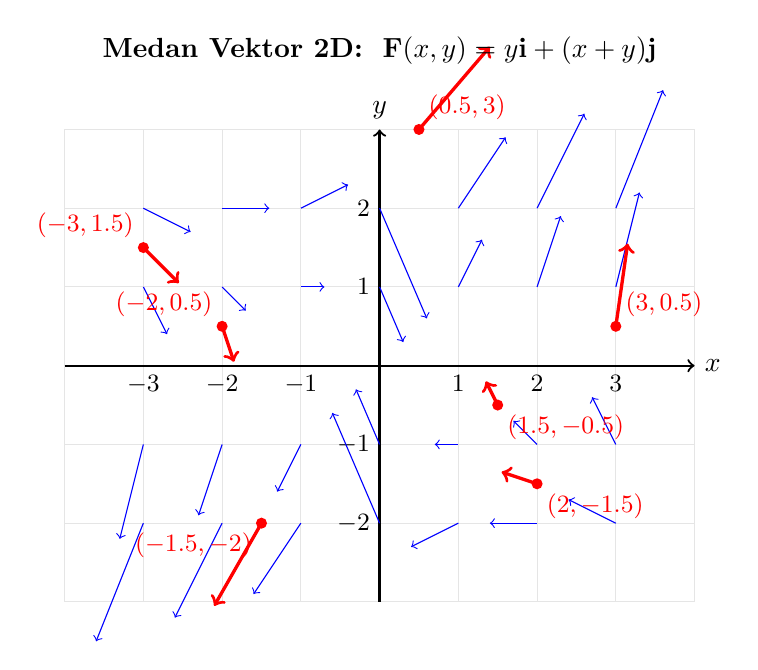
\begin{tikzpicture}[scale=1.0]
        \draw[gray!20, step=1] (-4,-3) grid (4,3);
        
        \draw[thick,->] (-4,0) -- (4,0) node[right] {$x$};
        \draw[thick,->] (0,-3) -- (0,3) node[above] {$y$};

        \foreach \x in {-3,-2,-1,1,2,3}
            \node[below] at (\x,0) {\small $\x$};
        \foreach \y in {-2,-1,1,2}
            \node[left] at (0,\y) {\small $\y$};
        
        \foreach \x in {-3,-2,-1,1,2,3}
        \foreach \y in {-2,-1,1,2}
        {
            \pgfmathsetmacro{\vx}{\y}
            \pgfmathsetmacro{\vy}{\x+\y}
            \draw[->,blue] (\x,\y) -- (\x+0.3*\vx,\y+0.3*\vy);
        }
        
        \draw[->,blue] (0,-2) -- (-0.6,-0.6);
        \draw[->,blue] (0,-1) -- (-0.3,-0.3);
        \draw[->,blue] (0,1) -- (0.3,0.3);
        \draw[->,blue] (0,2) -- (0.6,0.6);
        
        \draw[->,red,very thick] (-3,1.5) -- (-2.55,1.05);
        \draw[->,red,very thick] (-1.5,-2) -- (-2.1,-3.05);
        \draw[->,red,very thick] (0.5,3) -- (1.4,4.05);
        \draw[->,red,very thick] (1.5,-0.5) -- (1.35,-0.2);
        \draw[->,red,very thick] (3,0.5) -- (3.15,1.55);
        \draw[->,red,very thick] (-2,0.5) -- (-1.85,0.05);
        \draw[->,red,very thick] (2,-1.5) -- (1.55,-1.35);
        
        \fill[red] (-3,1.5) circle (2pt) node[above left] {\small $(-3,1.5)$};
        \fill[red] (-1.5,-2) circle (2pt) node[below left] {\small $(-1.5,-2)$};
        \fill[red] (0.5,3) circle (2pt) node[above right] {\small $(0.5,3)$};
        \fill[red] (1.5,-0.5) circle (2pt) node[below right] {\small $(1.5,-0.5)$};
        \fill[red] (3,0.5) circle (2pt) node[above right] {\small $(3,0.5)$};
        \fill[red] (-2,0.5) circle (2pt) node[above left] {\small $(-2,0.5)$};
        \fill[red] (2,-1.5) circle (2pt) node[below right] {\small $(2,-1.5)$};
        
        \node[above] at (0,3.7) {\textbf{Medan Vektor 2D: } $\mathbf{F}(x,y) = y\mathbf{i} + (x+y)\mathbf{j}$};
    \end{tikzpicture}
    \end{center}

    Vektor dua dimensi ditulis sebagai:

    \(\mathbf{F}(x, y) = P(x, y)\mathbf{i} + Q(x, y)\mathbf{j}\)

    Dengan soal:

    \(\mathbf{F}(x, y) = y\mathbf{i} + (x + y)\mathbf{j}\)

    Maka:

    \(P(x, y) = y, \quad Q(x, y) = x + y\)

    \begin{itemize}
      \item $P(x, y)$ adalah komponen arah \textbf{sumbu-$x$ (horizontal)},
      \item $Q(x, y)$ adalah komponen arah \textbf{sumbu-$y$ (vertikal)}.
    \end{itemize}

    Dari sketsa vektor, dapat dikatakan:

    \begin{enumerate}[itemsep=1em,leftmargin=*]
      \item \(x\), arah horizontal (sumbu-$x$) bergantung pada $y$.
      \item \(y\), arah vertikal (sumbu-$y$) bergantung pada $x$ dan $y$.
    \end{enumerate}

  \end{enumerate}
  \item Gunakan Crammar Rule untuk menyelesaikan (LO2, max point = 30)
  \begin{flalign*}
  &2x_1 + x_2 - x_3 = 2 &&\\
  &5x_1 + 2x_2 - 2x_3 = 9 &&\\
  &3x_1 + x_2 + x_3 = 5 &&
  \end{flalign*}

  \begin{enumerate}
    \item Mencari determinannya terlebih dahulu dari matriks koefisien:
    \[
    A = \begin{vmatrix}
    a & b & c \\
    d & e & f \\
    g & h & i
    \end{vmatrix}
    \]

    determinannya dapat dihitung dengan rumus:

    \(det(A) = a(ei - fh) - b(di - fg) + c(dh - eg)\)

    \[
    D = \begin{vmatrix}
    2 & 1 & -1 \\
    5 & 2 & -2 \\
    3 & 1 & 1
    \end{vmatrix}
    \]

    \(D = 2(2 \cdot 1 - (-2) \cdot 1) - 1(5 \cdot 1 - (-2) \cdot 3) + (-1)(5 \cdot 1 - 2 \cdot 3)\)

    \(D = 2(2 + 2) - 1(5 + 6) - 1(5 - 6)\)

    \(D = 8 - 11 + 1 = -2\)

    \item Mencari determinan \(D_{x_1}\), \(D_{x_2}\), dan \(D_{x_3}\):
      \begin{enumerate}
        \item Mencari \(D_{x_1}\):
        \[
        D_{x_1} = \begin{vmatrix}
        2 & 1 & -1 \\
        9 & 2 & -2 \\
        5 & 1 & 1
        \end{vmatrix}
        \]

        \(D_{x_1} = 2(2 \cdot 1 - (-2) \cdot 1) - 1(9 \cdot 1 - (-2) \cdot 5) + (-1)(9 \cdot 1 - 2 \cdot 5)\)

        \(D_{x_1} = 2(2 + 2) - 1(9 + 10) - 1(9 - 10)\)

        \(D_{x_1} = 8 - 19 + 1 = -10\)

        \item Mencari \(D_{x_2}\):
        \[
        D_{x_2} = \begin{vmatrix}
        2 & 2 & -1 \\
        5 & 9 & -2 \\
        3 & 5 & 1
        \end{vmatrix}
        \]

        \(D_{x_2} = 2(9 \cdot 1 - (-2) \cdot 5) - 2(5 \cdot 1 - (-2) \cdot 3) + (-1)(5 \cdot 5 - 9 \cdot 3)\)

        \(D_{x_2} = 2(9 + 10) - 2(5 + 6) - 1(25 - 27)\)

        \(D_{x_2} = 38 - 22 + 2 = 18\)

        \item Mencari \(D_{x_3}\):
        \[
        D_{x_3} = \begin{vmatrix}
        2 & 1 & 2 \\
        5 & 2 & 9 \\
        3 & 1 & 5
        \end{vmatrix}
        \]

        \(D_{x_3} = 2(2 \cdot 5 - 9 \cdot 1) - 1(5 \cdot 5 - 9 \cdot 3) + 2(5 \cdot 1 - 2 \cdot 3)\)

        \(D_{x_3} = 2(10 - 9) - 1(25 - 27) + 2(5 - 6)\)

        \(D_{x_3} = 2 - (-2) + 2(-1) = 2 + 2 - 2 = 2\)
      \end{enumerate}
      \item Mencari nilai \(x_1\), \(x_2\), dan \(x_3\) dengan rumus Cramer's Rule:

      \(x_1 = \frac{D_{x_1}}{D}, \quad x_2 = \frac{D_{x_2}}{D}, \quad x_3 = \frac{D_{x_3}}{D}\)

      \(x_1 = \frac{-10}{-2} = 5, \quad x_2 = \frac{18}{-2} = -9, \quad x_3 = \frac{2}{-2} = -1\) 

      \vspace{1em}
    
      Jadi, nilai dari \(x_1\), \(x_2\), dan \(x_3\) adalah:

      \(x_1 = 5, \quad x_2 = -9, \quad x_3 = -1\)
  \end{enumerate}

  \item Gunakan Gauss-Jordan untuk menyelesaikan (LO2, max point = 30)
  \begin{flalign*}
  &2x_1 + x_2 - x_3 = 2 &&\\
  &5x_1 + 2x_2 - 2x_3 = 9 &&\\
  &3x_1 + x_2 + x_3 = 5 &&
  \end{flalign*}

  \begin{enumerate}
    \item Membuat augmented matrix dari sistem persamaan linear:
    \[
    \left[\begin{array}{ccc|c}
    2 & 1 & -1 & 2 \\
    5 & 2 & -2 & 9 \\
    3 & 1 & 1 & 5
    \end{array}\right]
    \]
    \item Melakukan operasi baris elementer untuk mengubah augmented matrix ke bentuk reduced row echelon form (RREF):
    \begin{enumerate}
      \item Membuat pivot pertama = 1 dengan membagi baris pertama dengan 2:
      
      \(R_1 = \frac{1}{2}R_1\)

      \(R_1 = \frac{1}{2}[2, 1, -1 \vert 2]\)

      \(R_1 = [1, \frac{1}{2}, -\frac{1}{2} \vert 1]\)

      \[
      \left[\begin{array}{ccc|c}
      1 & \frac{1}{2} & -\frac{1}{2} & 1 \\
      5 & 2 & -2 & 9 \\
      3 & 1 & 1 & 5
      \end{array}\right]
      \]
      \item Mengeliminasi elemen di bawah pivot pada kolom pertama:

      \(R_2 = R_2 - 5R_1\)

      \(R_2 = [5, 2, -2 \vert 9] - 5[1, \frac{1}{2}, -\frac{1}{2} \vert 1]\)

      \(R_2 = [5 - 5, 2 - \frac{5}{2}, -2 + \frac{5}{2} \vert 9 - 5]\)

      \(R_2 = [0, -\frac{1}{2}, \frac{1}{2} \vert 4]\)

      \vspace{1em}

      \(R_3 = R_3 - 3R_1\)

      \(R_3 = [3, 1, 1 \vert 5] - 3[1, \frac{1}{2}, -\frac{1}{2} \vert 1]\)

      \(R_3 = [3 - 3, 1 - \frac{3}{2}, 1 + \frac{3}{2} \vert 5 - 3]\)

      \(R_3 = [0, -\frac{1}{2}, \frac{5}{2} \vert 2]\)


      \[
      \left[\begin{array}{ccc|c}
      1 & \frac{1}{2} & -\frac{1}{2} & 1 \\
      0 & -\frac{1}{2} & \frac{1}{2} & 4 \\
      0 & -\frac{1}{2} & \frac{5}{2} & 2
      \end{array}\right]
      \]
      \item Membuat pivot kedua = 1 dengan mengalikan baris kedua dengan \(-2\):
      
      \(R_2 = -2R_2\)

      \(R_2 = -2[0, -\frac{1}{2}, \frac{1}{2} \vert 4]\)

      \(R_2 = [0, 1, -1 \vert -8]\)

      \[
      \left[\begin{array}{ccc|c}
      1 & \frac{1}{2} & -\frac{1}{2} & 1 \\
      0 & 1 & -1 & -8 \\
      0 & -\frac{1}{2} & \frac{5}{2} & 2
      \end{array}\right]
      \]

      \item Mengeliminasi elemen di atas dan bawah pivot pada kolom kedua:
      
      \(R_1 = R_1 - \frac{1}{2}R_2\)

      \(R_1 = [1, \frac{1}{2}, -\frac{1}{2} \vert 1] - \frac{1}{2}[0, 1, -1 \vert -8]\)

      \(R_1 = [1, \frac{1}{2} - \frac{1}{2}, -\frac{1}{2} + \frac{1}{2} \vert 1 + 4]\)

      \(R_1 = [1, 0, 0 \vert 5]\)

      \vspace{1em}

      \(R_3 = R_3 + \frac{1}{2}R_2\)

      \(R_3 = [0, -\frac{1}{2}, \frac{5}{2} \vert 2] + \frac{1}{2}[0, 1, -1 \vert -8]\)

      \(R_3 = [0, -\frac{1}{2} + \frac{1}{2}, \frac{5}{2} - \frac{1}{2} \vert 2 - 4]\)

      \(R_3 = [0, 0, 2 \vert -2]\)

      \[
      \left[\begin{array}{ccc|c}
      1 & 0 & 0 & 5 \\
      0 & 1 & -1 & -8 \\
      0 & 0 & 2 & -2
      \end{array}\right]
      \]
      \item Membuat pivot ketiga = 1 dengan membagi baris ketiga dengan 2:
      
      \(R_3 = \frac{1}{2}R_3\)

      \(R_3 = \frac{1}{2}[0, 0, 2 \vert -2]\)

      \(R_3 = [0, 0, 1 \vert -1]\)

      \[
      \left[\begin{array}{ccc|c}
      1 & 0 & 0 & 5 \\
      0 & 1 & -1 & -8 \\
      0 & 0 & 1 & -1
      \end{array}\right]
      \]
      \item Mengeliminasi elemen di atas pivot pada kolom ketiga:
      
      \(R_2 = R_2 + R_3\)

      \(R_2 = [0, 1, -1 \vert -8] + [0, 0, 1 \vert -1]\)

      \(R_2 = [0, 1, 0 \vert -9]\)

      \[
      \left[\begin{array}{ccc|c}
      1 & 0 & 0 & 5 \\
      0 & 1 & 0 & -9 \\
      0 & 0 & 1 & -1
      \end{array}\right]
      \]

      \item Jadi, nilai-nilai variablenya adalah:
      \[x_1 = 5, \quad x_2 = -9, \quad x_3 = -1\]
    \end{enumerate}
  \end{enumerate}
\end{enumerate}

Referensi:

\begin{itemize}
  \item Lecture Note 7.
  \item \url{https://tutorial.math.lamar.edu/classes/calciii/VectorFields.aspx}
  \item \url{https://math.libretexts.org/Bookshelves/Calculus/Supplemental_Modules_%28Calculus%29/Vector_Calculus/4%3A_Integration_in_Vector_Fields/4.3%3A_Line_Integrals}
  \item \url{https://math.libretexts.org/Bookshelves/Precalculus/Precalculus_(Stitz-Zeager)/08%3A_Systems_of_Equations_and_Matrices/8.05%3A_Determinants_and_Cramers_Rule}
  \item \url{https://math.libretexts.org/Bookshelves/Applied_Mathematics/Applied_Finite_Mathematics_(Sekhon_and_Bloom)/02%3A_Matrices/2.02%3A_Systems_of_Linear_Equations_and_the_Gauss-Jordan_Method}
\end{itemize}

\end{document}
